\documentclass[11pt]{article}
\usepackage[margin=1in]{geometry} 
\usepackage{amsmath,amsthm,amssymb}
\usepackage{mathtools}
\usepackage{tikz}
\usetikzlibrary{positioning,arrows}
%\usepackage{tikz-berge}
%\usepackage{algorithm}
%\usepackage[noend]{algpseudocode}

 
\newcommand{\N}{\mathbb{N}}
\newcommand{\Z}{\mathbb{Z}}
\newcommand{\R}{\mathbb{R}}
\renewcommand{\'}{^{'}}
 
\newenvironment{theorem}[2][Theorem]{\begin{trivlist}
\item[\hskip \labelsep {\bfseries #1}\hskip \labelsep {\bfseries #2.}]}{\end{trivlist}}
\newenvironment{lemma}[2][Lemma]{\begin{trivlist}
\item[\hskip \labelsep {\bfseries #1}\hskip \labelsep {\bfseries #2.}]}{\end{trivlist}}
\newenvironment{definition}[2][Definition]{\begin{trivlist}
\item[\hskip \labelsep {\bfseries #1}\hskip \labelsep {\bfseries #2.}]}{\end{trivlist}}
\newenvironment{problem}[2][Problem]{\begin{trivlist}
\item[\hskip \labelsep {\bfseries #1}\hskip \labelsep {\bfseries #2.}]}{\end{trivlist}}
\newenvironment{question}[2][Question]{\begin{trivlist}
\item[\hskip \labelsep {\bfseries #1}\hskip \labelsep {\bfseries #2.}]}{\end{trivlist}}

\begin{document}
\title{Chapter 1}
\author{Zachary Campbell}

\maketitle

\begin{section}{Bipartite graphs and matchings}

	Throughout this thesis we will be interested in a specific subclass of graphs known as 
	bipartite graphs. Unless otherwise noted, our algorithms will assume a bipartite structure.

	\begin{definition}{(Bipartite graph)}
		A \emph{bipartite graph} is a graph whose vertices can be partitioned into two 
		set $L$ and $R$ such that all edges connect a vertex $l\in L$ to a vertex $r\in R$.
		We will denote this graph $G = (L,R,E)$, where $E$ is the edge set.
	\end{definition}
	
	\begin{figure}[h]
		\centering
	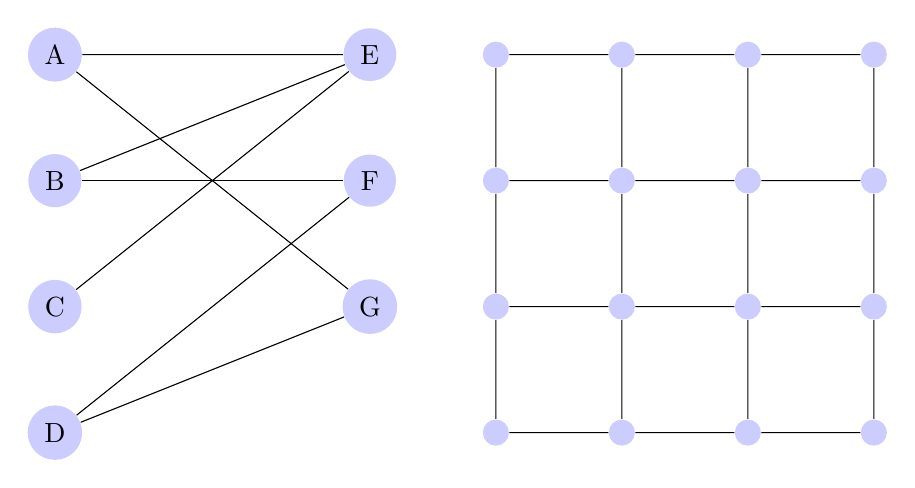
\begin{tikzpicture}[scale=.8,auto=left,every node/.style={circle,fill=blue!20}]
		%left nodes
		\node (n1) at (1,10) {A};
		\node (n2) at (1,8) {B};
		\node (n3) at (1,6) {C};
		\node (n4) at (1,4) {D};

		%right nodes
		\node (n5) at (6,10) {E};
		\node (n6) at (6, 8) {F};
		\node (n7) at (6, 6) {G};
		
		%edges
		\draw (n1) -- (n5);
		\draw (n1) -- (n7);
		\draw (n2) -- (n5);
		\draw (n2) -- (n6);
		\draw (n3) -- (n5);
		\draw (n4) -- (n6);
		\draw (n4) -- (n7);

		%left nodes
		\node (n1) at (8,10) {};
		\node (n2) at (8,8) {};
		\node (n3) at (8,6) {};
		\node (n4) at (8,4) {};

		%center left nodes
		\node (n5) at (10,10) {};
		\node (n6) at (10,8) {};
		\node (n7) at (10,6) {};
		\node (n8) at (10,4) {};

		%center right nodes
		\node (n9) at (12,10) {};
		\node (n10) at (12,8) {};
		\node (n11) at (12,6) {};
		\node (n12) at (12,4) {};

		%right nodes
		\node (n13) at (14,10) {};
		\node (n14) at (14,8) {};
		\node (n15) at (14,6) {};
		\node (n16) at (14,4) {};

		%edges
		\draw (n1) -- (n2);
		\draw (n1) -- (n5);
		\draw (n2) -- (n3);
		\draw (n2) -- (n6);
		\draw (n3) -- (n4);
		\draw (n3) -- (n7);
		\draw (n4) -- (n8);
		\draw (n5) -- (n6);
		\draw (n5) -- (n9);
		\draw (n6) -- (n7);
		\draw (n6) -- (n10);
		\draw (n7) -- (n8);
		\draw (n7) -- (n11);
		\draw (n8) -- (n12);
		\draw (n9) -- (n10);
		\draw (n9) -- (n13);
		\draw (n10) -- (n11);
		\draw (n10) -- (n14);
		\draw (n11) -- (n12);
		\draw (n11) -- (n15);
		\draw (n12) -- (n16);
		\draw (n13) -- (n14);
		\draw (n14) -- (n15);
		\draw (n15) -- (n16);
	\end{tikzpicture}
	\caption{Examples of bipartite graphs}
	\end{figure}

	In Figure 1 we have a bipartite graph with vertex partition given by $L = \{A,B,C,D\}$ and 
	$R = \{E,F,G\}$. All edges in this graph are between a node $l\in L$ and a node $r\in R$. The 
	graph on the right is also bipartite. It may take a little more time to convince yourself that 
	you can partition the vertices into disjoint $L$ and $R$ in a way that maintains the 
	bipartite property. Try it!

	Now that we know what we are working with, let's introduce a problem that 
	we'd like to solve on these graphs.
	We now describe the notion of a matching on a graph. We will define it for arbitrary graphs, 


	\begin{definition}{(Matching)}
		Let $G = (V,E)$ be a graph. A subset $M\subset E$ is a \emph{matching} if no two 
		edges in $M$ are incident to the same vertex.
	\end{definition}

	We say that a vertex $v\in V$ is matched with respect to $M$ if it is an endpoint of some 
	edge in $M$. The following figure shows some examples of different matchings on one of the 
	graphs from Figure 1.

	\begin{figure}[h]
		\centering
		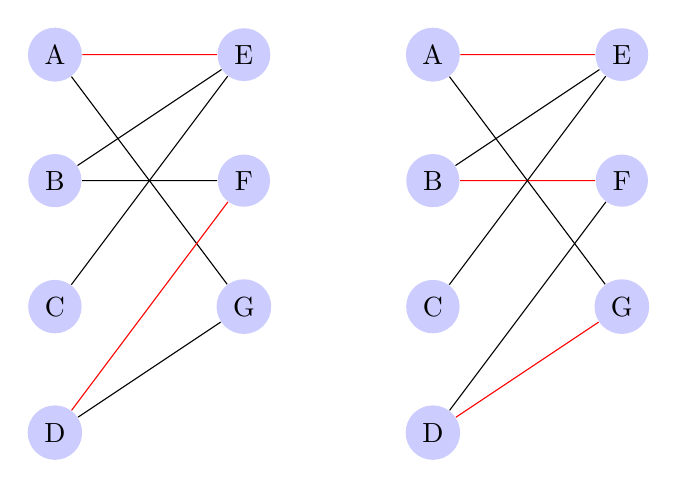
\begin{tikzpicture}[scale=.8,auto=left,every node/.style={circle,fill=blue!20}]
		
		%left nodes
		\node (n1) at (1,10) {A};
		\node (n2) at (1,8) {B};
		\node (n3) at (1,6) {C};
		\node (n4) at (1,4) {D};

		%right nodes
		\node (n5) at (4,10) {E};
		\node (n6) at (4, 8) {F};
		\node (n7) at (4, 6) {G};
		
		%edges
		\draw[red] (n1) -- (n5);
		\draw (n1) -- (n7);
		\draw (n2) -- (n5);
		\draw (n2) -- (n6);
		\draw (n3) -- (n5);
		\draw[red] (n4) -- (n6);
		\draw (n4) -- (n7);

		%left nodes
		\node (m1) at (7,10) {A};
		\node (m2) at (7,8) {B};
		\node (m3) at (7,6) {C};
		\node (m4) at (7,4) {D};

		%right nodes
		\node (m5) at (10,10) {E};
		\node (m6) at (10, 8) {F};
		\node (m7) at (10, 6) {G};
		
		%edges
		\draw[red] (m1) -- (m5);
		\draw (m1) -- (m7);
		\draw (m2) -- (m5);
		\draw[red] (m2) -- (m6);
		\draw (m3) -- (m5);
		\draw (m4) -- (m6);
		\draw[red] (m4) -- (m7);

		\end{tikzpicture}
		\caption{Examples of matchings on a bipartite graph}
	\end{figure}

	There many different valid matchings on the graph in Figure 2. Oftentimes, we want to find 
	the largest matching on a graph. (ADD SENTENCE OR TWO ON MOTIVATION FOR MAXIMAL MATCHING.)
	This leads to the following definition.

	\begin{definition}{(Maximal matching)}
		A \emph{maximal matching} on $G$ is a matching $M$ such that if any other edge 
		not in $M$ is added to $M$, it is no longer a valid matching. Alternatively put, 
		$M$ is maximal if there is no matching $M\'$ such that $M\subset M\'$.
	\end{definition}

	Both matchings in Figure 2 are maximal matchings; in each case there are no edges that 
	we can add to $M$ and have that $M$ is still a matching. However, notice that the size of 
	the matchings is different, even though both are maximal on $G$. This leads to the following 
	definition.

	\begin{definition}{(Maximum matching)}
		A matching $M$ on a graph $G$ is said to be a maximum matching if for all other 
		matchings $M\'$ on $G$, $|M\'| \leq |M|$.
	\end{definition}

	In our example, the matching on the right given by $M = \{(A,E), (B,F), (D,G)\}$ is a 
	maximum matching (convince yourself). In general there may be many unique maximum matchings 
	on a graph.\\
	In this section we are interested in general methods for finding maximum matchings on 
	bipartite graphs. One of the fundamental approaches is to look at certain subgraphs called 
	alternating paths. Before we define what these are, let's look at a motivating example.
	Suppose we have the matching on the left in Figure 2. So $M = \{(A,E),(D,F)\}$. Consider 
	the following sequence of vertices in the graph:

	\begin{figure}[h]
		\centering
		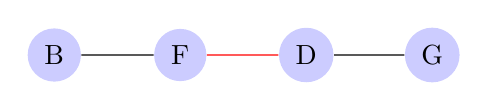
\begin{tikzpicture}[scale=.8,auto=left,every node/.style={circle,fill=blue!20}]

			\node (n1) at (1,10) {B};
			\node (n2) at (3,10) {F};
			\node (n3) at (5,10) {D};
			\node (n4) at (7,10) {G};

			\draw (n1) -- (n2); 
			\draw[red] (n2) -- (n3);
			\draw (n3) -- (n4);
		\end{tikzpicture}
	\end{figure}

	Call this sequence $p$. Let's perform an 
	operation that we will denote $M\oplus p$, which operates like XOR: add to $M$ each edge in 
	$p$ that isn't in $M$, and remove from $M$ each edge in $p$ that is in $M$. This gives us 
	the following segment:

	\begin{figure}[h]
		\centering
		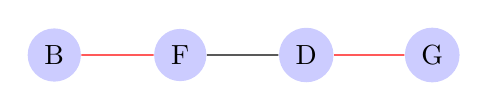
\begin{tikzpicture}[scale=.8,auto=left,every node/.style={circle,fill=blue!20}]

			\node (n1) at (1,10) {B};
			\node (n2) at (3,10) {F};
			\node (n3) at (5,10) {D};
			\node (n4) at (7,10) {G};

			\draw[red] (n1) -- (n2); 
			\draw (n2) -- (n3);
			\draw[red] (n3) -- (n4);
		\end{tikzpicture}
	\end{figure}

	Notice that the size of our matching has grown by 1! In fact, this new matching is exactly 
	the matching given by the graph on the right in Figure 2. This is a general technique in 
	finding maximum matchings. We want to look for these paths that start and end at unmatched 
	vertices, and whose edges are alternately matched and unmatched. If we can find one of these 
	paths, we will be able to increase the size of matching. We define this formally now.

	\begin{definition}{(Alternating path)}
		Let $G$ be a graph and $M$ some matching on $G$. An \emph{alternating path} is a 
		sequence of vertices and edges that begins with an unmatched vertex, and whose 
		edges alternate between being in $M$ and not in $M$.
	\end{definition}

	\begin{definition}{(Augmenting path)}
		An \emph{augmenting path} is an alternating path that starts and ends on unmatched 
		vertices. When we augment $M$ by an augmenting path $p$, we use the notation 
		$M\oplus p$.
	\end{definition}



\end{section}
\end{document}
